\documentclass[tikz,border=8pt]{standalone}
\usepackage[T1]{fontenc}
\usepackage{lmodern}
\usetikzlibrary{arrows.meta,backgrounds,fit,positioning,shadows.blur}

\definecolor{humanblue}{HTML}{2563EB}
\definecolor{sensorcyan}{HTML}{0891B2}
\definecolor{datagreen}{HTML}{059669}
\definecolor{twinpurple}{HTML}{7C3AED}
\definecolor{actionorange}{HTML}{EA580C}
\definecolor{futuregray}{HTML}{64748B}

\begin{document}
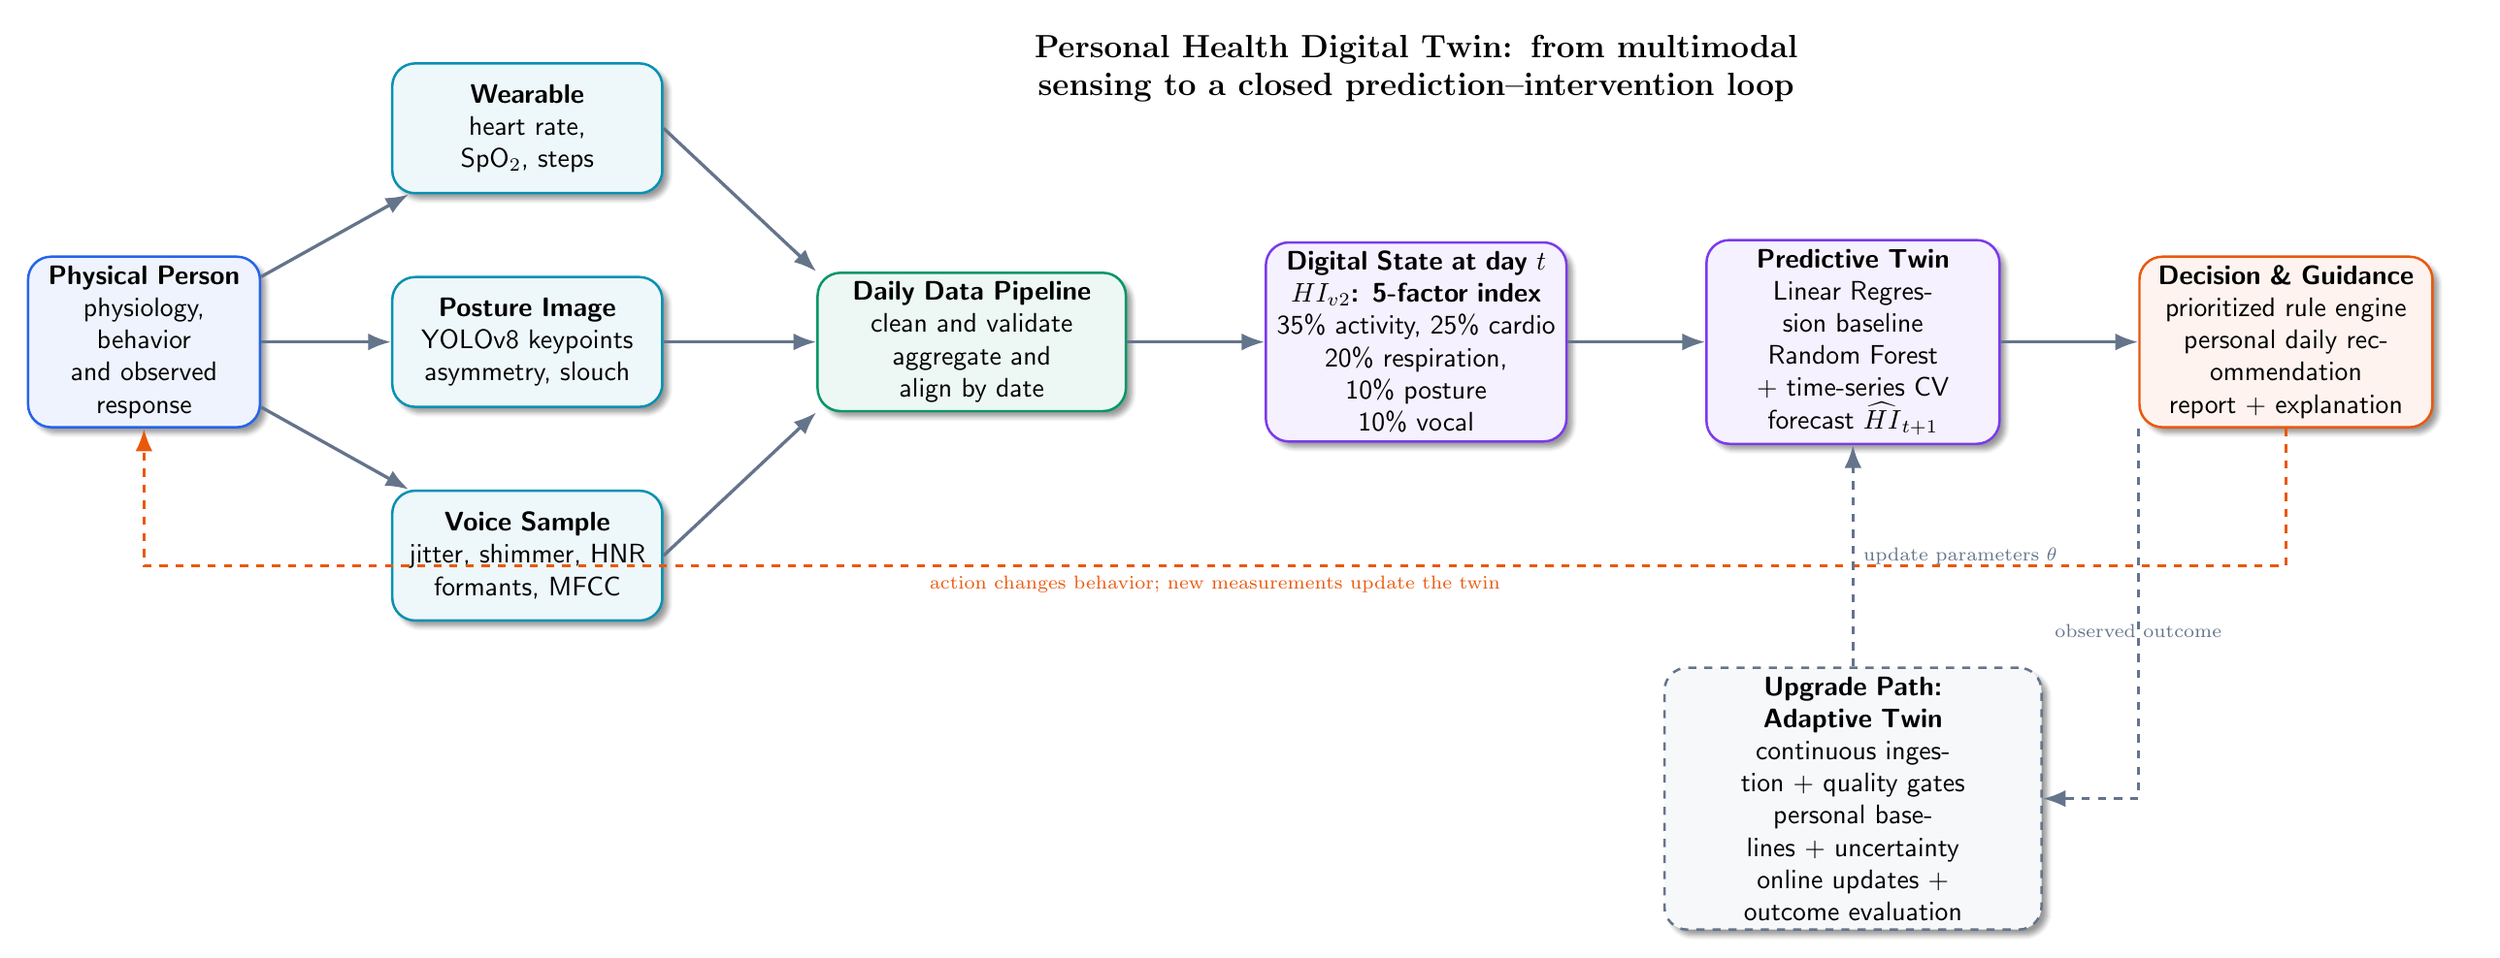
\begin{tikzpicture}[
  font=\sffamily,
  >=Latex,
  flow/.style={-{Latex[length=3mm]}, very thick, draw=futuregray},
  feedback/.style={-{Latex[length=3mm]}, very thick, dashed, draw=actionorange},
  box/.style={rounded corners=3mm, minimum height=17mm, align=center,
              text width=33mm, draw, line width=.9pt, fill=white,
              blur shadow={shadow blur steps=5}},
  source/.style={box, draw=sensorcyan, fill=sensorcyan!7},
  process/.style={box, draw=datagreen, fill=datagreen!7},
  twin/.style={box, draw=twinpurple, fill=twinpurple!7},
  action/.style={box, draw=actionorange, fill=actionorange!7},
  title/.style={font=\bfseries\large, align=center},
  note/.style={font=\scriptsize, align=center, text=futuregray}
]

% The physical person and multimodal observations
\node[box, draw=humanblue, fill=humanblue!8, text width=28mm] (human)
  {\textbf{Physical Person}\\physiology, behavior\\and observed response};

\node[source, above right=8mm and 17mm of human] (wearable)
  {\textbf{Wearable}\\heart rate, SpO$_2$, steps};
\node[source, right=17mm of human] (posture)
  {\textbf{Posture Image}\\YOLOv8 keypoints\\asymmetry, slouch};
\node[source, below right=8mm and 17mm of human] (voice)
  {\textbf{Voice Sample}\\jitter, shimmer, HNR\\formants, MFCC};

\node[process, right=20mm of posture, text width=38mm] (prep)
  {\textbf{Daily Data Pipeline}\\clean and validate\\aggregate and align by date};

\node[twin, right=18mm of prep, text width=37mm] (state)
  {\textbf{Digital State at day $t$}\\\textbf{$HI_{v2}$: 5-factor index}\\35\% activity, 25\% cardio\\20\% respiration, 10\% posture\\10\% vocal};

\node[twin, right=18mm of state, text width=36mm] (predict)
  {\textbf{Predictive Twin}\\Linear Regression baseline\\Random Forest + time-series CV\\forecast $\widehat{HI}_{t+1}$};

\node[action, right=18mm of predict, text width=36mm] (recommend)
  {\textbf{Decision \& Guidance}\\prioritized rule engine\\personal daily recommendation\\report + explanation};

% Primary data and decision flow
\draw[flow] (human) -- (wearable);
\draw[flow] (human) -- (posture);
\draw[flow] (human) -- (voice);
\draw[flow] (wearable.east) -- (prep.north west);
\draw[flow] (posture.east) -- (prep.west);
\draw[flow] (voice.east) -- (prep.south west);
\draw[flow] (prep) -- (state);
\draw[flow] (state) -- (predict);
\draw[flow] (predict) -- (recommend);

% Closed-loop intervention: the key digital-twin idea
\draw[feedback] (recommend.south) -- ++(0,-18mm) -|
  node[pos=.25, below, note, text=actionorange]{action changes behavior; new measurements update the twin}
  (human.south);

% Current implementation boundary
\begin{scope}[on background layer]
  \node[draw=twinpurple!55, dashed, rounded corners=5mm, inner sep=5mm,
        fill=twinpurple!2, fit=(prep)(state)(predict)(recommend),
        label={[title, text=twinpurple]above:Implemented Health Digital Twin}] {};
\end{scope}

% Future adaptive layer
\node[box, dashed, draw=futuregray, fill=futuregray!5, text width=47mm,
      below=29mm of predict] (future)
  {\textbf{Upgrade Path: Adaptive Twin}\\continuous ingestion + quality gates\\personal baselines + uncertainty\\online updates + outcome evaluation};
\draw[flow, dashed] (future.north) -- node[right, note]{update parameters $\theta$} (predict.south);
\draw[flow, dashed] (recommend.south west) |- node[near start, below, note]{observed outcome} (future.east);

\node[title, above=17mm of state, text width=120mm]
  {Personal Health Digital Twin: from multimodal sensing to a closed prediction--intervention loop};

\end{tikzpicture}
\end{document}
